\documentclass[12pt]{article}

\usepackage[utf8]{inputenc}
\usepackage{color}
\usepackage{graphicx}
\usepackage{amsmath}
\usepackage{amssymb}
\usepackage{amsthm}

\title{Manual Básico de LaTeX}
\author{
	Elyas Correa Nogueira\\
	\and
	Fabiana Silva Finoti\\
	\and
	Isabela Daiana Pereira\\
	\and
	Israel Mateus Melo Oliveira\\	
}
\date{6 de Maio de 2019}

\begin{document}
	
	\maketitle
	
	\newpage
	
	\section{Introdução}
		O Latex (estilizado como \LaTeX) é um sistema de preparação de documentos desenvolvido nos anos 80 pelo americano Leslie Lamport. Amplamente empregado na fabricação de documentos, o LaTeX utiliza texto simples para a confecção dos arquivos, fazendo a formatação do texto (\textit{itálico}, \textbf{negrito} {\color{red} cores}) por meio de marcadores, de maneira que o escritor foque no conteúdo ao invés da estilização.
	
		A padronização dos documentos oferecidos pelo LaTeX faz com que ele seja preferencial na fabricação de vários documentos acadêmicos, eliminando assim erros na formatação de tais documentos. Neste manual, será abordada a estrutura básica de um documento TeX e vários pacotes que oferecem funcionalidades importantes para quem está escrevendo o documento.
	
	\section{Como utilizar o LaTeX?}
	
		\subsection{Instalação em Linux e Windows}
		
			\subsubsection{Instalação em Ubuntu}
				Para facilitar o processo, será explicado como instalar o LaTeX em um sistema Ubuntu. Abra o terminal e digite a seguinte linha:\\\\
				\texttt{sudo apt-get install texlive texlive-latex-extra texlive-lang-portuguese}\\
			
				Assim, será instalado em seu computador os pacotes necessários para compilar arquivos básicos .tex. Para o uso de ferramentas mais complexas, pode ser necessária a instalação de outros pacotes -- como o \texttt{texlive-math-extra}, usado para matemática complexa. 
			
				Uma vez que os pacotes de compilação foram instalados, você precisará de um editor para começar a sua aventura LaTeX. Para respeitar o que foi utilizado em aula, é recomendado que você use o TeXstudio. Para instalá-lo, abra o terminal e digite:\\\\
				\texttt{sudo apt-get install texstudio}
			
			\subsubsection{Instalação em Windows}
				No Windows, a instalação dos compiladores e do editor podem ser feitas por meio do browser. Entre no link \texttt{https://miktex.org/download}, tenha certeza que você está na aba do Windows e clique no botão de Download (o site oferece um tutorial passo-a-passo em caso de dúvidas). Quando o arquivo for baixado, abra o instalador, faça bom uso do 'Avançar' e espere o fim do processo.
			
				Agora que os compiladores estão instalados, chegou a hora do editor. Entre no link \texttt{http://texstudio.sourceforge.net/}, clique na aba de Downloads, ache a versão correspondente ao seu Windows e espere o fim do download. Abra o instalador e vá clicando em 'Avançar' até que o TeXstudio esteja instalado em seu computador.
			
		\subsection{Criação de Documento Básico}
			Nessa subseção, você será apresentado a um código básico de LaTeX e as linhas serão explicadas posteriormente.
			
			\begin{figure}[h]
				\begin{center}
					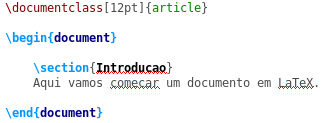
\includegraphics{codigo1.png}
				\end{center}
			\end{figure}
		
			Na primeira linha, o escritor declara que o documento digitado será do tipo \textit{article}, ou seja, seguirá os padrões de formatação de um artigo acadêmico, com \texttt{12pt} sendo o tamanho da fonte utilizada.
			A linha seguinte aponta que o documento começará a ser escrito, abrindo assim um bloco que contém todas as informações que serão utilizadas.
		    
			O LaTeX organiza os tópicos em seções. Sendo assim, o usuário consegue distribuir todos as seções do documento desejado utilizando o marcador da imagem.
		    
		    
		\subsection{Estrutura de Documento}
			A linguagem LaTeX funciona a base de comandos que são iniciados com $\backslash$ que é um marcador. Os comandos são escritos nas formas $\backslash$comando ou $\backslash$begin\{{comando}\}...$\backslash$end\{{comando}\}. Quando vem escrito nesta última forma, ele é chamado de ambiente. O texto de cada tipo de documento começa com $\backslash$begin\{{document}\} e termina com $\backslash$end\{{document}\}. Tudo o que vem antes disso é considerado o preâmbulo e tudo o que vem depois de $\backslash$end\{{document}\} é ignorado. É no preâmbulo que são colocadas todas as informações referentes às principais características que terá seu documento. Começa com $\backslash$documentclass\{{estilo}\}. No lugar de estilo é colocado o nome de um dos estilos pré-definidos, segue alguns exemplos:
			\begin{itemize}
				\item \textbf {article}: Textos pequenos;
				\item \textbf {report}: Relatórios;
				\item \textbf {book}:  Livros, apostilas;
				\item \textbf {letters}: Cartas.
			\end{itemize}
			Os estilos não são apenas estes. Geralmente congressos, universidades e outros meios disponibilizam outros estilos de formatação para apresentação de trabalhos. Isso mostra uma das vantagens do LaTeX, que é a flexibilidade para se criar novas formatações que atendem a diferentes necessidades.
			Podendo, também, ser selecionadas algumas opções dentro do estilo escolhido, como:
			\begin{itemize}
				\item \textbf {Tamanho}: Padrão da letra: 11pt ou 12pt(pontos), o último é usado com mais frequência;
				\item \textbf {twoside}: Que imprime em ambos os lados da página;
				\item \textbf {oneside}: Imprime em um só lado da página;
				\item \textbf {twocolumn}: Produz o texto disposto em duas colunas na página;
				\item \textbf {onecolumn}: Produz o texto disposto em uma coluna;
				\item \textbf {landscape}: Produz uma página na forma de paisagem;
				\item \textbf {eqno}: Isto faz com que a numeração das fórmulas sejam colocadas a esquerda em vez
				de a direita;
				\item \textbf {fleqn}: Faz com que a fórmula fique localizada na margem esquerda em vez de estar centralizada;
				\item \textbf {openright}: Faz com que os capítulos sejam iniciados apenas nas páginas ímpares;
				\item \textbf {openany}: Permite que os capítulos sejam iniciados nas páginas ímpar ou par;
				\item \textbf {Tamanho da folha}: Pode ser a4, letterpaper, etc.
			\end{itemize}
			
			Essas opções são colocadas entre colchetes sem espaço entre as palavras e com vírgula. Exemplo:\\
			$\backslash$documentstyle\{[twocolumn,12pt,a4]{article}\} \\
			
			Abaixo segue alguns comandos utizados para a estrutura básica do documento:
			
			
			\begin{itemize}
				\item $\backslash$usepackage\{{pacote}\} : Comando utilizado no início do arquivo para utilizar os pacotes disponíveis;
				\item $\backslash$begin\{{document}\}: Comando utilizado para iniciar o arquivo;
				\item $\backslash$end\{{document}\} : Comando utilizado para terminar o arquivo.
			\end{itemize}
		
		
		\subsection{Matemática}
			A Matemática é a ciência que relaciona as práticas do cotidiano e a natureza ao raciocínio humano e à lógica numérica.
			As fórmulas matemáticas podem ser digitadas tanto no meio de um texto ou em destaque:
			
			\subsubsection{Fórmulas no meio do texto}
			
			Tem que ser usado \$...\$ para que a equação apareça no meio do texto.
			Exemplo: 
			Segunda a equação \texttt{\$a \^\ \{{2}\}= b \^\ \{{2}\} + c \^\ \{{2}\}\$} concluímos que:\\
			\textbf{Resultado: }Segundo a equação $a^{2}= b^{2}+c^{2}$ concluímos que:
			
			\subsubsection{Fórmulas em destaque}
				Utiliza-se o comando \texttt{$\backslash$begin\{{equation}\}/$\backslash$end\{{equation}\}}, conforme exemplo a seguir:\\
				Segundo a equação:\\
				\texttt{begin \{{equation}\}} 
				
				\texttt{\$a \^\ \{{2}\}= b \^\ \{{2}\} + c \^\ \{{2}\} \$} \\
				\texttt{$\backslash$end\{{equation}\}} \\
				podemos concluir que: \\
				\textbf{Resultado: }Segundo a equação:
				\begin{equation}
					a^{2}= b^{2}+c^{2}
				\end{equation}
				podemos concluir que:
			
			\subsubsection{Subescritos e Sobrescritos}
				Sobrescrito – É feito usando: b \^\ \{{e}\} onde b é a base e e o expoente.\\
				Ex: 2 \^\ \{{5}\} = $2^{5}$ \\
				Subescrito – É feito usando: b\_\ \{{i}\} onde b é a base e i o índice.
				Ex: 2 \_\ \{{5}\} = $2_{5}$
				
			\subsubsection{Frações}
				Podem ser feita usando:
				\begin{itemize}
					\item $\backslash$ \\
					Exemplo: (a+b)/2 = $(a + b)/2$
					\item $\backslash$frac\{{numerador}\}\{{denominador}\}
					Exemplo: \\ $\backslash$frac\{{(a + b)}\}\{{2}\} = $\frac{(a + b)}{2}$
				\end{itemize}
			
			\subsubsection{Raízes}
				São feitas usando:  $\backslash$sqrt[]\{{}\} Exemplo: $\sqrt[3]{8}$ \\
				Se for omitido o termo [ ] automaticamente a raíz será quadrada.
				
			\subsubsection{Símbolos}
				O LaTeX possui vários símbolos para montar fórmulas como integrais, somatórios, letras especiais, entre outros. Seguem exemplos a seguir:\\
				$\backslash$int = $\int$\\
				$\backslash$exists = $\exists$ \\
				$\backslash$infty = $\infty$
			
			\subsubsection{Funcões}
				O LaTeX também possui símbolos de funções.Exemplos:\\
				$\backslash$log10 = $\log10$ \\
				$\backslash$sin60 = $\sin60$
			
			\subsubsection{Espaçamento nas Fórmulas}
				No modo matemático o TeX ignora os espaços dados colocando o espaço que convêm a ele, mas como alguns autores gostam de mudar isso há alguns comandos especiais de espaçamento:
				\begin{itemize}
					\item $\backslash$, pequeno espaço 
					\item $\backslash$; grande espaço 
					\item $\backslash$: médio espaço 
					\item $\backslash$! espaço negativo(backspace) 
				\end{itemize}
				É bom deixar o TEX colocar o espaço que ele quer, mas como nem tudo é perfeito deve-se ficar atento quando houver símbolos de integral, derivada, raízes e quocientes, pois geralmente o TEX confunde a estrutura lógica. \\
				Exemplo: ydx é visto como o produto de três variáveis pelo TEX, logo quando digitar isso coloque espaço para que se compreenda que é uma derivada  y$\backslash$,dx = y\,dx .
		
		\subsection{Imagens}
			Imagens como diferentes tipos de arquivos (pdf, png, jpg, or gif) podem ser inseridas no documento. É preciso que as imagens inseridas estejam no mesmo local do arquivo .tex quando for compilar o documento. 
			Imagens são elementos essenciais na maioria dos documentos científicos. L A T E X oferece várias opções para manipular imagens e torná-las exatamente do que você precisa. Neste artigo é explicado como incluir imagens nos formatos mais comuns, como encolher, ampliar e rotacioná-los e como referenciá-los em seu documento.
			
			Um exemplo sobre como importar uma imagem:
			\begin{figure} [h]
				\centering
				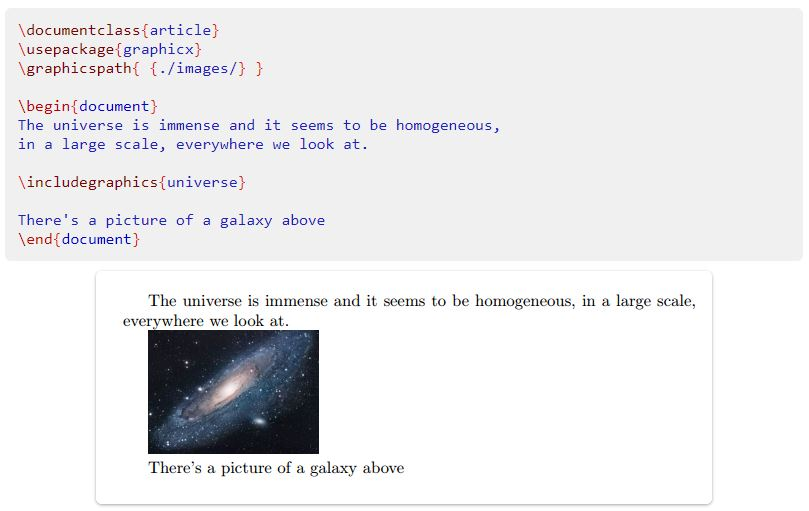
\includegraphics[scale=0.9]{21.JPG}
			\end{figure}
			
			\pagebreak
			Se quisermos especificar melhor como L A T E X deve incluir nossa imagem no documento (comprimento, altura, etc), podemos passar essas configurações no seguinte formato:
			\begin{figure} [h]
				\centering
				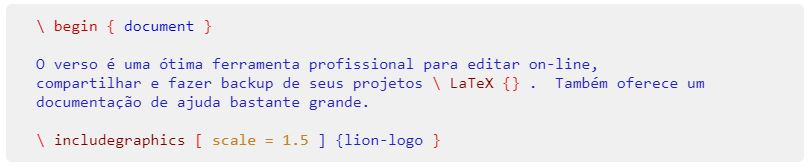
\includegraphics[scale=0.9]{22.JPG}
			\end{figure}
			\begin{figure} [h]
				\centering
				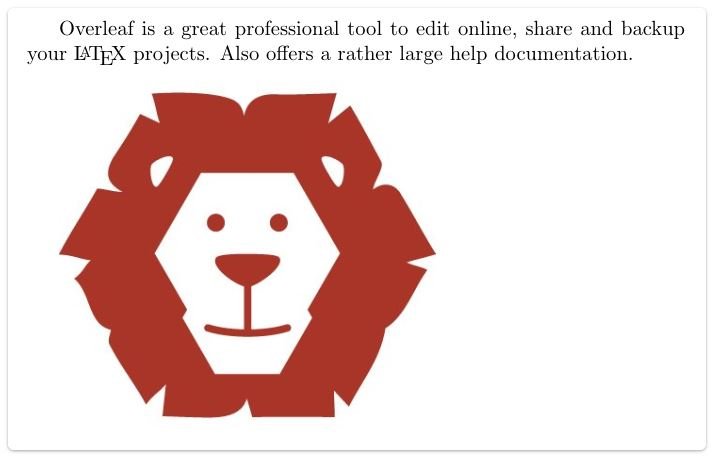
\includegraphics[scale=0.8]{23.JPG}
			\end{figure}
			\pagebreak
			
			O comando:
			\begin{figure} [h]
				\centering
				
\includegraphics[scale=0.9]{24.JPG}
			\end{figure}
			
			
			incluirá a imagem lion-logo no documento, a scale=1.5 parâmetro extra scale=1.5 fará exatamente isso, dimensionará a imagem 1.5 do seu tamanho real.
			
			Você também pode dimensionar a imagem para uma largura e altura específicas.
			\begin{figure} [h]
				\centering
				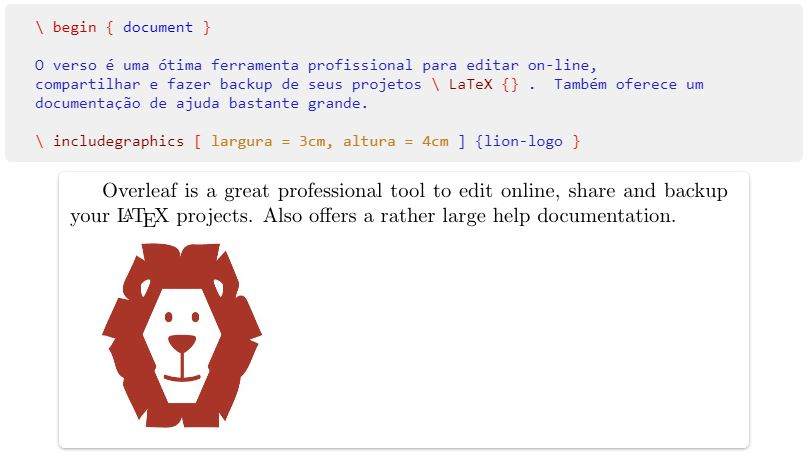
\includegraphics[scale=0.9]{25.JPG}
			\end{figure}
			
		
		\subsection{Tabela de Conteúdos}
			Gerar um índice pode ser feito com alguns comandos simples. O LaTeX usará os cabeçalhos de seção para criar o índice e há comandos para criar uma lista de figuras e uma lista de tabelas também. A seguir um exemplo de código para criar um índice:
			\begin{figure} [h]
				\centering
				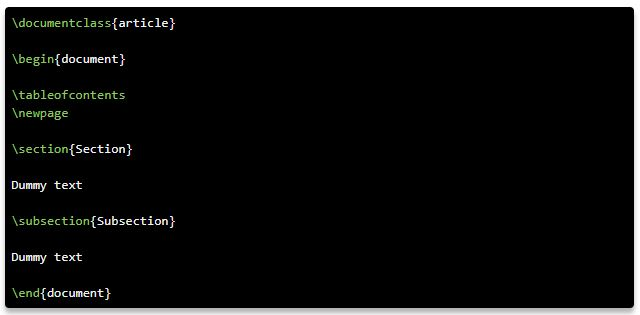
\includegraphics[scale=0.9]{26.JPG}
			\end{figure}
			
			Depois de compilar o arquivo .tex duas vezes, você obterá o seguinte índice:
			
			\begin{figure} [h]
				\centering
				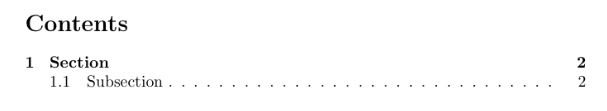
\includegraphics[scale=0.9]{28.JPG}
			\end{figure}
			\pagebreak
			A geração de uma lista de figuras e tabelas funciona da mesma maneira. A seguir, um exemplo da adição de uma figura fictícia e uma tabela para colocar as listas no apêndice do documento:
			\begin{figure} [h]
				\centering
				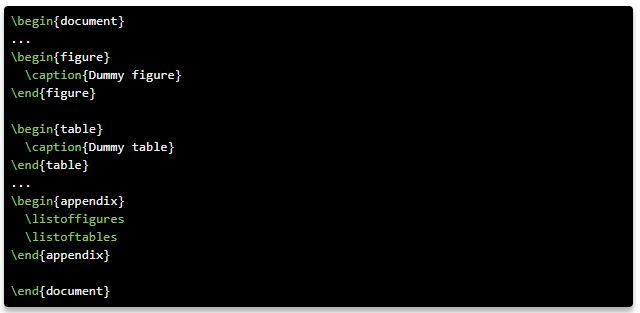
\includegraphics[scale=0.9]{27.JPG}
			\end{figure}
			
			
			Depois de compilar duas vezes novamente, as listas serão geradas da seguinte maneira:
			\begin{figure} [h]
				\centering
				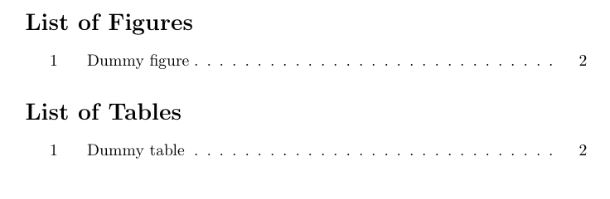
\includegraphics[scale=0.9]{29.JPG}
			\end{figure}
			\pagebreak
			
			Às vezes, faz sentido mostrar apenas um subconjunto dos títulos de todas as seções ou de uma seção específica. Por esta razão, você pode definir uma deflexão usando o comando \ setcounter {tocdepth} {X}, onde X é a profundidade desejada. Um valor de 0 significa que seu índice mostrará nada e 5 significa que os parágrafos serão mostrados. O valor deve ser definido no preâmbulo do documento e aplicado automaticamente ao documento inteiro:
			\begin{figure} [h]
				\centering
				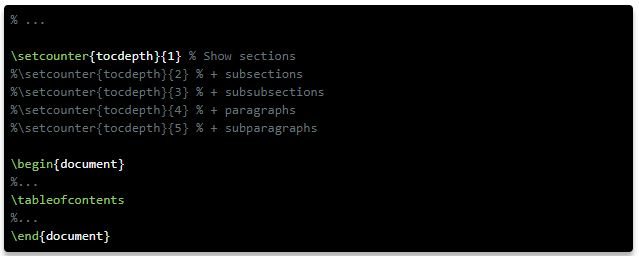
\includegraphics[scale=0.9]{30.JPG}
			\end{figure}
			
			Usando o exemplo acima, a configuração tocdepth = 1 levará à seguinte saída:
			\begin{figure} [h]
				\centering
				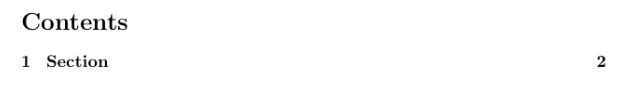
\includegraphics[scale=0.9]{31.JPG}
			\end{figure}
			\pagebreak
			
			Você pode facilmente aumentar a verbosidade do seu índice, definindo a profundidade como algo, o que levaria à seguinte saída:
			\begin{figure} [h]
				\centering
				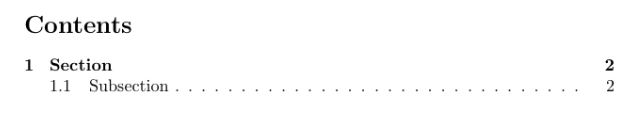
\includegraphics[scale=0.9]{32.JPG}
			\end{figure}
			
			Se você não quiser alterar a profundidade de todas as seções, também poderá ajustar a profundidade de cada seção individualmente. Neste caso, você não precisa definir a profundidade de corte antes da seção, que deve ter mais ou menos profundidade.
			\begin{figure} [h]
				\centering
				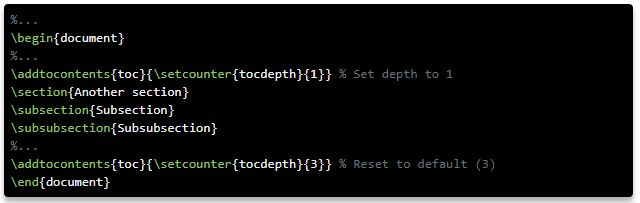
\includegraphics[scale=0.9]{33.JPG}
			\end{figure}
			
			Isso gerará o índice a seguir para esta seção:
			\begin{figure} [h]
				\centering
				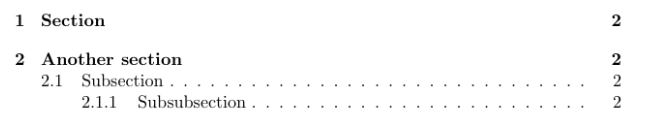
\includegraphics[scale=0.9]{34.JPG}
			\end{figure}
			\pagebreak
		
		\subsection{Bibliografia}
			Referências bibliográficas são geralmente mantidas em um arquivo de bibliografia cuja extensão é .bib, este arquivo consiste em uma lista de registros e campos . Cada registro bibliográfico contém informações relevantes para uma única entrada.
			\begin{figure} [h]
				\centering
				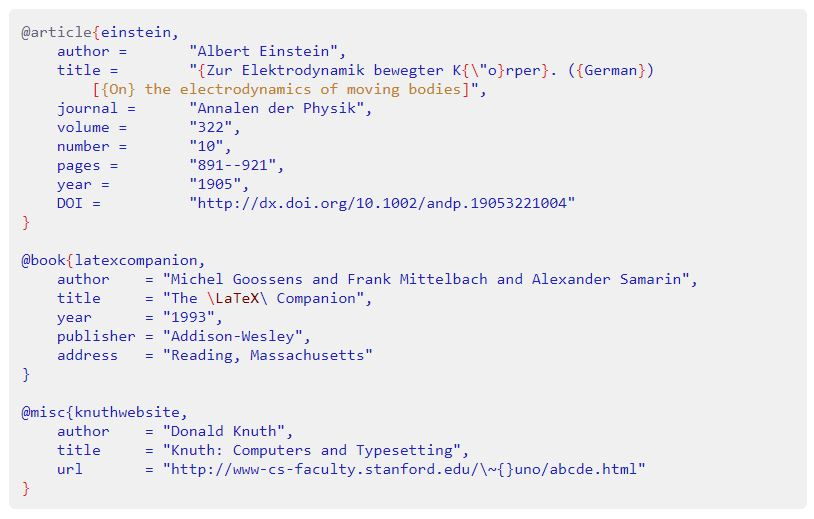
\includegraphics[scale=0.9]{35.JPG}
			\end{figure}
			\pagebreak
			
			Este arquivo contém registros em um formato especial, por exemplo, a primeira referência bibliográfica é definida por:
			
			\textbf{@article{...}}:
			Esta é a primeira linha de uma entrada de registro, @article indica o tipo de entrada e informa ao BibTeX que as informações armazenadas aqui são sobre um artigo. Além dos tipos de entrada mostrados no exemplo ( article , book e misc ).
			
			\textbf{Einstein:}
			O rótulo einstein é atribuído a essa entrada, é um identificador que pode ser usado para referenciar este artigo dentro do documento.
			
			\textbf{Author = "Albert Einstein"}:
			Este é o primeiro campo na entrada da bibliografia, indica que o autor deste artigo é Albert Einstein. Vários campos separados por vírgulas podem ser adicionados usando a mesma sintaxe key = value , por exemplo: title, pages, year, URL, etc.
		
		\subsection{Notas de Rodapé}
			Uma nota de rodapé pode ser inserida após a palavra ou frase a qual se refere através do comando:
			\begin{figure}[h]
				\centering
				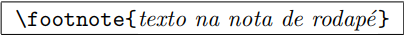
\includegraphics[scale=0.5]{no.png}
			\end{figure}
			
			O número é opcional, e pode ser usado para forçar um determinado numero ao invés do automático que seria gerado pelo compilador o texto é o que vai aparecer na nota no final da página.\\
			Exemplo:
			\begin{figure}[h]
				\centering
				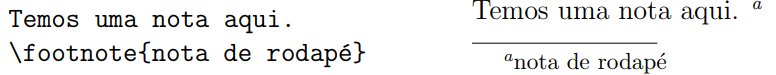
\includegraphics[scale=0.45]{xx.png}
			\end{figure}
		
		\subsection{Tabelas}
		
				\subsubsection{Tabular}
					Uma tabela pode ser especificada pelo ambiente tabular. É possível utilizar linhas horizontais e verticais sem se preocupar com a largura das colunas que é calculada automaticamente pelo LATEX. A criação de uma tabela é feita da seguinte forma:
					\begin{figure}[h]
						\centering
						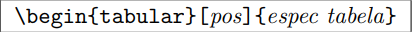
\includegraphics[scale=0.45]{t.png}
					\end{figure}
		
					O argumento \textit{espec} especifica a quantidade e alinhamentos das colunas:
					\begin{itemize}
						\item \textbf{$|$}: adiciona uma linha vertical;
						\item \textbf{l}: indica uma coluna alinhada `a esquerda;
						\item \textbf{r}: indica uma coluna alinhada `a direita;
						\item \textbf{c}: indica uma coluna com texto centralizado;
						\item \textbf{p\{{largura}\}}: indica uma coluna especial com texto justificado capaz de quebrar linhas, com a largura especificada com unidade de medida.
					\end{itemize}
					Para mesclar colunas de células podemos usar o comando\\
					$\backslash$multicolumn\{{num}\}\{{formato}\}{\{texto}\}
					que concatena o número de colunas especificado por \textit{num} com o alinhamento especificado por \textit{formato} e possui como conteúdo \textit{texto}.\\ 
					Uma tabela pode ser inserida dentro do ambiente \textit{table} o que faz dela um objeto flutuante. Vantagens de utilizar esse tipo de ambiente é a posição correta da tabela no texto, sem que seja quebrada em das páginas, por exemplo, faz com que a tabela apareça em um índice de tabelas e também a inserção de rótulos e legendas.
					O argumento \textit{pos} especifica a posição vertical da tabela relativamente à linha base do texto envolvente. Use as letras \textit{t}, \textit{b}, \textit{c} e \textit{p} para especificar o alinhamento da tabela no topo, fundo, centro ou em uma página especial contendo somente objetos flutuantes respectivamente. \textit{!} é usado para  ignora alguns parâmetros internos.\\
					Dentro de um ambiente tabular, o \& salta para a próxima coluna, $\backslash$$\backslash$
					inicia uma nova linha e $\backslash$hline insere uma linha horizontal. Pode adicionar
					linhas parciais usando $\backslash$cline{j-i}, onde j e i são os números das colunas
					de onde e para onde a linha se deve estender.
					\\
					A seguir apresentamos uma tabela criada como objeto flutuante:
					\begin{table}[ht]
						\begin{center}
							\begin{tabular}{|c|r|l|}
								\hline
								Centro & Direita & Esquerda \\
								\hline
								\hline
								\multicolumn{3}{|c|}{Números}\\
								\hline
								1 & 2 & 3 \\ \cline{2-3}
								4 & 5 & 6 \\
								\hline
							\end{tabular}
							\caption{Uma tabela simples}
						\end{center}
					\end{table}
		
		
		
					Agora, apresentamos os códigos utilizados para gerar a Tabela 1 mostrada:\\
					\texttt{$\backslash$begin\{{table}\}[ht]\\}
					\texttt{$\backslash$begin\{{center}\}\\}
					\texttt{$\backslash$begin\{{tabular}\}{\{$|$c$|$r$|$l$|$}\}\\}
					\texttt{$\backslash$hline\\}
					\texttt{Centro \& Direita \& Esquerda \\}
					\texttt{$\backslash$hline \\}
					\texttt{$\backslash$hline\\}
					\texttt{$\backslash$multicolumn\{{3}\}{\{$|$c$|$}\}{\{Números}\}\\}
					\texttt{$\backslash$hline \\}
					\texttt{1 \& 2 \& 3 $\backslash$$\backslash$ $\backslash$cline\{{2-3}\}\\
						4 \& 5 \& 6 \\}
					\texttt{$\backslash$hline \\}
					\texttt{$\backslash$end\{{tabular}\}\\}
					\texttt{$\backslash$caption\{{Uma tabela simples}\}\\}
					\texttt{$\backslash$end\{{center}\}\\}
					\texttt{$\backslash$end\{{table}\}\\}
		
					Para mesclar facilmente as linhas das células podemos usar o pacote
					\textit{multirow} que possui o comando $\backslash$multirow que funciona de maneira análoga
					ao $\backslash$multicolumn, sendo que é possível passar como posição um *, indicando
					que o compilador deve procurar pelo melhor ajuste, e é preciso deixar a posição correspondente da coluna cujas linhas estão sendo mescladas em branco.\\
					Um pequeno exemplo:\\
		
					\begin{center}
						\begin{tabular}{|c|r|r|l|}
							\hline
							Centro & Direita & Direita & Esquerda \\
							\hline
				
							& 4 & 5 & 6 \\
							\hline
						\end{tabular}
					\end{center}
					O código do exemplo mostrado:\\
					\texttt{$\backslash$begin\{{tabular}\}\{{$|$c$|$r$|$r$|$l$|$}\}\\}
					\texttt{$\backslash$hline \\}
					\texttt{Centro \& Direita \& Direita \& Esquerda \\}
					\texttt{$\backslash$hline\\}
					\texttt{$\backslash$multirow\{{2}\}\{{*}\}\{{Números}\} \& 1 \& 2 \& 3 \\}
					\texttt{\& 4 \& 5 \& 6 \\}
					\texttt{$\backslash$hline}
					\texttt{$\backslash$end\{{tabular}\}}
		
				\subsubsection{Table}	
		
					O ambiente \textit{table} possibilita a inclusão de uma legenda para a tabela e trabalha a mesma como um objeto flutuante. A sintaxe deste ambiente é
		
					\begin{figure}[h]
						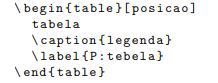
\includegraphics[scale=0.7]{a.png}
					\end{figure}
					Onde posição é o parâmetro que indica onde a tabela deve ser preferencialmente inserida, tabela corresponde ao código da tabela a ser inserida, $\backslash$caption é o comando correspondente a legenda e legenda é o texto a ser apresentado como legenda, $\backslash$label é o comando para referência cruzada como já apresentado.
					Exemplo contendo uma tabela e o código correspondente:
					\begin{figure}[h]
						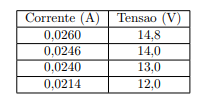
\includegraphics[scale=0.7]{q.png}
					\end{figure}
					\begin{figure}[h]
						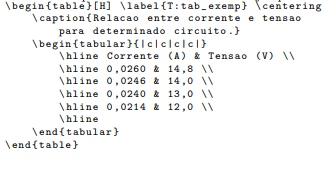
\includegraphics[scale=0.7]{qq.png}
					\end{figure}
		
		\subsection{Geração automática de Tabelas}
			Para se gerar uma tabela automaticamente, basta visitar o site \texttt{http://tablesgenerator.com/}. Este site, possui a seguinte interface:
			
			\begin{figure}[h]
				\centering
				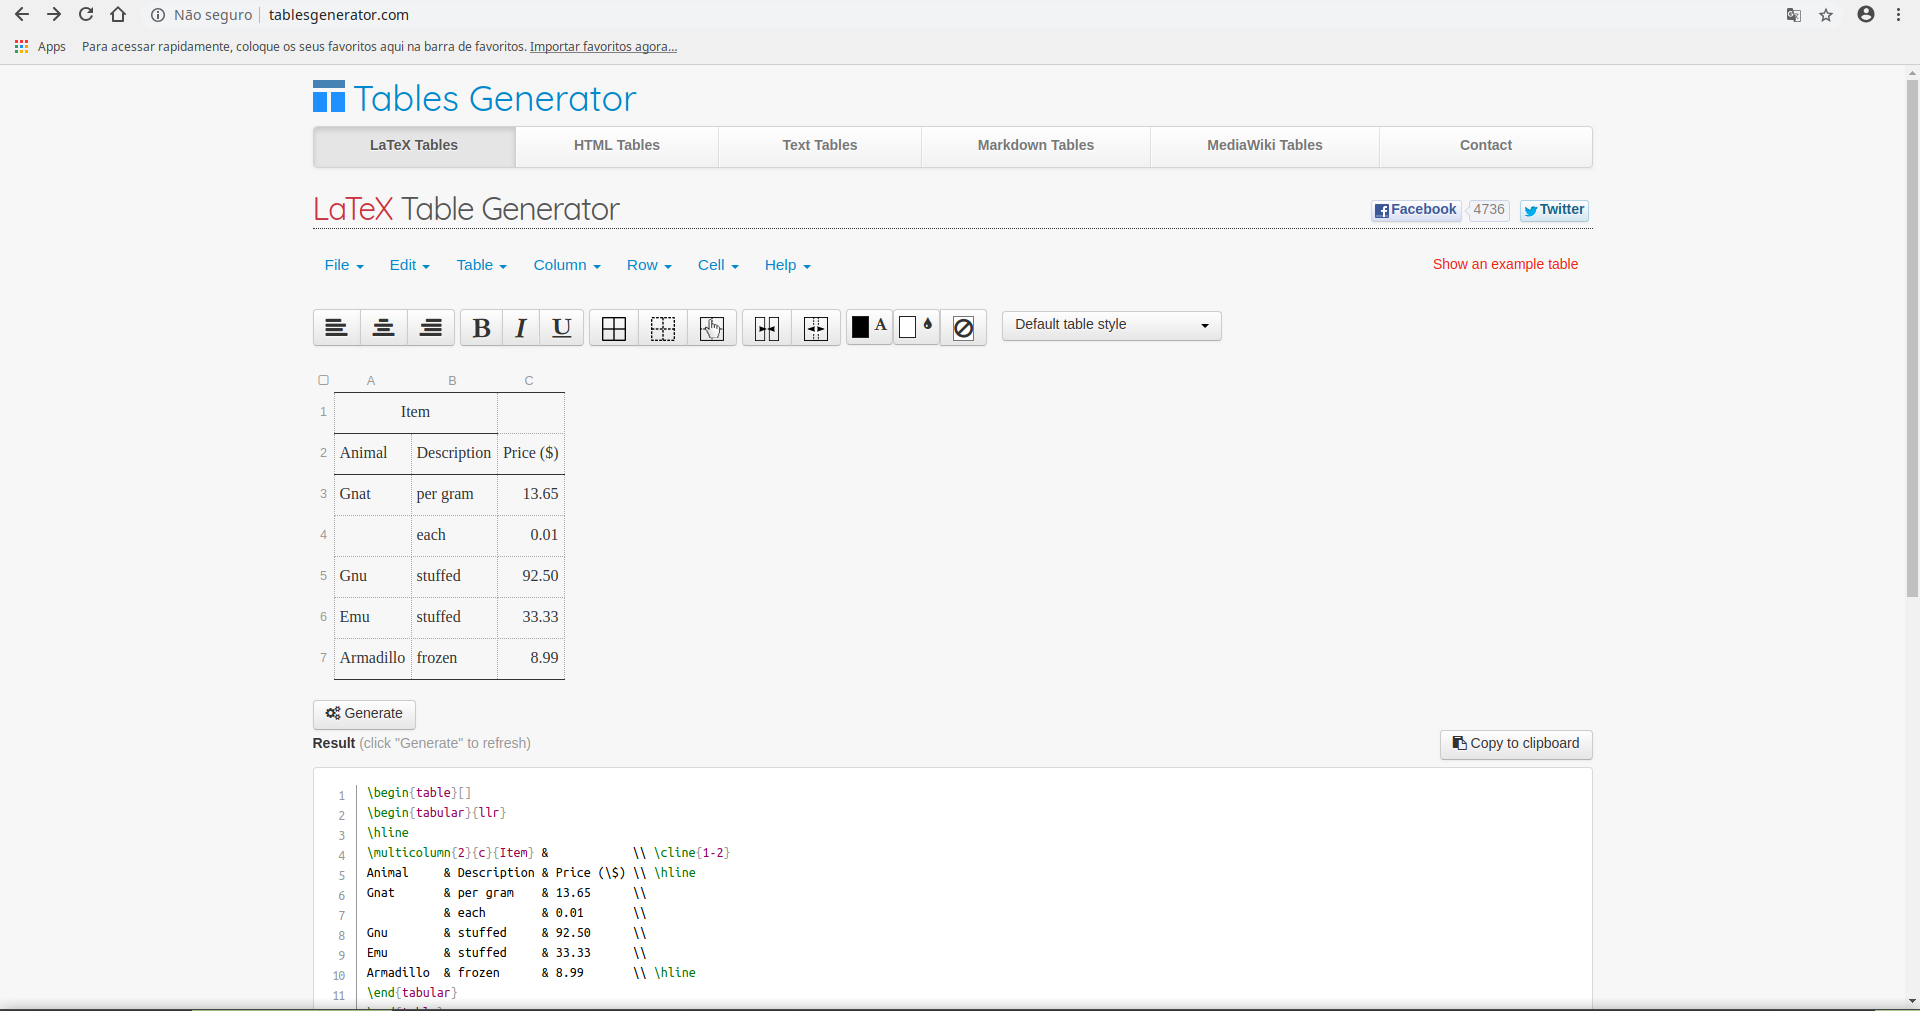
\includegraphics[scale=0.1]{ca.png}
			\end{figure}
			
			Neste gerador de tabelas, basta digitar a conteúdo desejado que ele gera o código correspondente em latex.
		
			
	\section{Pacotes}
		O LaTeX define um conjunto básico de macros para edição de textos. Caso o usuário queira usar alguma função mais complexa o LaTeX permite que ele inclua arquivos com novos macros. Esses arquivos são chamados de pacotes. Existem pacotes para escrever colorido, para incluir figuras, incluir pseudo-código etc. O usuário pode até criar seu próprio pacote. Para incluir um pacote no texto basta digitar a linha:
	
		\begin{figure}[h]
			\centering
			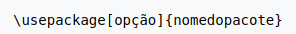
\includegraphics[scale=0.6]{pa.png}
		\end{figure}	
	
		\subsection{aa}
			O pacote aa foi desenvolvido pelo jornal francês Astronomy $\&$ Astrophysics para padronizar os artigos que são enviados para publicação. Esse pacote pode ser baixado por meio do link \\\texttt{http://ftp.edpsciences.org/pub/aa/readme.html} e seu uso garante que toda a formatação do documento digitado seguirá os padrões requeridos para publicação pela AA.
			
			Uma vez que o pacote foi inserido na pasta do arquivo TEX, o usuário pode definir o modelo que ele deseja, podendo escolher entre o formato padrão (\texttt{$\backslash$documentclass$\{aa\}$}), de uma coluna (\texttt{$\backslash$documentclass[onecolumn]$\{aa\}$}) ou com adaptação para uma lista extensa de autores e instituições \\(\texttt{$\backslash$documentclass[longauth]$\{aa\}$}).
		
		\subsection{aastex}
			Seguindo o exemplo do pacote anterior, o AASTeX foi desenvolvido pela American Astronomical Society (AAS) para auxiliar os autores na preparação de artigos que serão submetidos ao jornal. O pacote foi feito para uso em LaTeX2e e pode ser baixado no link\\ \texttt{https://journals.aas.org/aastex-package-for-manuscript-preparation/}.
			
			Uma vez que o arquivo for baixado, você pode usar o pacote por meio da linha \texttt{$\backslash$documentclass[aastex62]}. Assim, o documento que for digitado seguirá os padrões da AAS.
			
			Entre as funcionalidades do AASTeX, é possível destacar os modelos de tabela que são oferecidos. O pacote usa um ambiente chamado \textit{deluxetable}, fortemente indicado para a construção de tabelas longas. O usuário pode escolher entre usar o modelo padrão do LaTeX e o modelo deluxe do AASTeX. Veja o \textit{deluxetable} em aplicação no seguinte exemplo:
			
			\begin{figure}[h]
				\begin{center}
					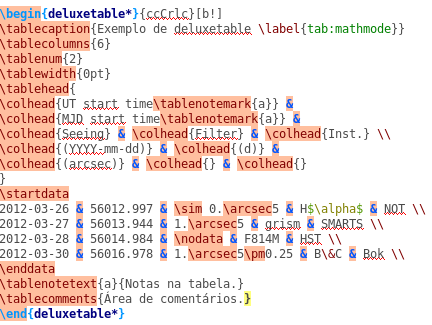
\includegraphics[scale=0.6]{tabelaAASTEX.png}
				\end{center}
			\end{figure}
		
			Assim como a table padrão do LaTeX, o deluxetable guia-se pela definição de "c", "l" e "r" para organizar o posicionamento das colunas. Entretanto, se o usuário estiver utilizando o AASTeX e definir o posicionamento com letras maiúsculas (como ele faz na terceira coluna), o modo Matemática é ativado automaticamente, dispensando assim o uso dos \$s no código. O resultado do código acima é:
			
			\begin{figure}[h]
				\begin{center}
					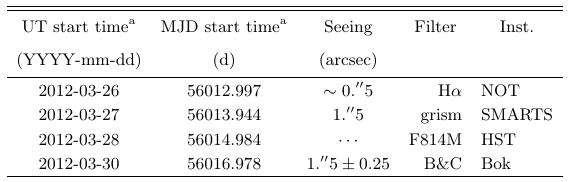
\includegraphics[scale=0.4]{rtabelaAASTEX.png}
				\end{center}
			\end{figure}
			\newpage
			
		
		\subsection{amsart}
			O pacote amsart é amplamente utilizado para publicações da American Mathematical Society, garantindo que o documento editado seguirá os padrões estabelecidos pelo jornal. Na maioria das versões de LaTeX, o pacote já está incluso e pode ser utilizado por meio da linha\\
			\texttt{$\backslash$documentclass[]$\{$amsart$\}$}\\
			Contudo, o pacote pode ser baixado por meio do link \texttt{https://ctan.org/pkg/amsart}, onde o arquivo contém diversos exemplos de como o pacote deve ser utilizado.
		
		\subsection{amscd}
			O pacote amscd, por sua vez, é utilizado para a criação de diagramas comutativos. O pacote, também desenvolvido pela AMS, possui a limitação de oferecer apenas diagramas retangulares, não tendo a capacidade de gerar setas diagonais ou funções mais exóticas.
			
			Para utilizar esse pacote, o usuário deve inserir a linha \texttt{$\backslash$usepackage$\{amscd\}$} e, caso seja necessário, o download do pacote pode ser feito por meio do link \texttt{https://ctan.org/pkg/amscd}. A seguir, um exemplo do código de um diagrama comutativo e seu resultado.
			
			\begin{figure}[h]
				\begin{center}
					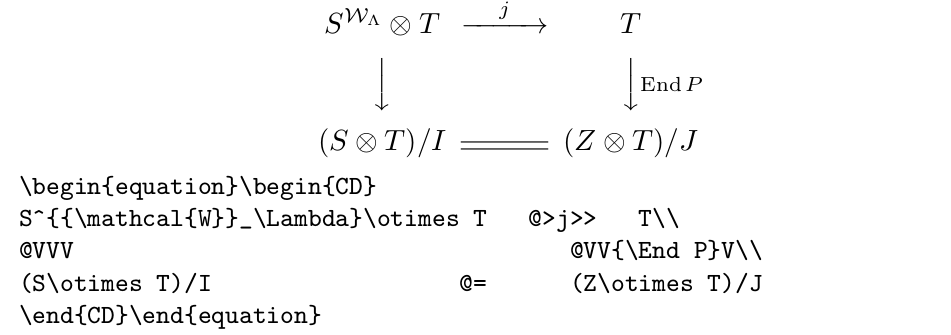
\includegraphics[scale=0.4]{amscd.png}
				\end{center}
			\end{figure}
			\newpage
			
		
		\subsection{amsfonts}
			Voltado para um leque de caracteres matemáticos, o pacote amsfonts carrega diversas variações de fontes já existentes (letras gregas e símbolos matemáticos subscritos), além de incluir novos caracteres (novos símbolos matemáticos e letras Fraktur).
			
			O pacote pode ser incluído através da linha \texttt{$\backslash$usepackage$\{amsfonts\}$} e pode ser baixado, junto com um manual de uso, através do link \texttt{https://ctan.org/pkg/amsfonts}.
		
		\subsection{amsmath}
			Considerado o pŕincipal pacote da distribuição AMS-LATEX, o amsmath é amplamente utilizado para digitação matemática na composição de um documento TEX. O pacote já está incluso na distribuição padrão e pode ser utilizado após a linha \texttt{$\backslash$usepackage$\{amsmath\}$}.
			
			Entre as funcionalidades desse pacote, o amsmath oferece um ambiente simples para estabelecer casos divergentes para uma equação, como nesse caso:
			
			\begin{equation} f(x) =
				\begin{cases}
					x& \text{se $x$ $\geqslant$ 0},\\
					-x& \text{se $x <$  0}.
				\end{cases}
			\end{equation}
			
			A codificação desse trecho é feita com as linhas:\\
			\texttt{$\backslash$begin$\{$equation$\}$ f(x) =}\\
			\texttt{$\backslash$begin$\{$cases$\}$}\\
			\texttt{x$\&$ $\backslash$text$\{$se $x$ $\$\backslash$geqslant$\$$  0$\}$,$\backslash\backslash$}\\
			\texttt{-x$\&$ $\backslash$text$\{$se $x <$  0$\}$.}\\
			\texttt{$\backslash$end$\{$cases$\}$}\\
			\texttt{$\backslash$end$\{$equation$\}$}
		
		\subsection{amssymb}
			O pacote amssymb inclui uma gama de símbolos matemáticos que podem ser utilizados no documento. Assim como o \textit{amsmath}, ele está incluso na distribuição original do \LaTeX e pode ser inserido por meio da linha \texttt{$\backslash$usepackage$\{amssymb\}$}.
			
			Os símbolos inclusos no pacote podem ser consultados no link\\ \texttt{http://milde.users.sourceforge.net/LUCR/Math/mathpackages/amssymb-symbols.pdf}.
			
			No subtópico anterior, foi utilizado um exemplo de amssymb com o uso do sinal de maior ou igual. O símbolo $\geqslant$ pode ser utilizado com o comando $\backslash$geqslant.
		
		\subsection{amsthm}
			O pacote amsthm oferece ao usuário uma versão melhorada do ambiente de teoremas padrão de \LaTeX. O amsthm insere ao \textit{$\backslash$newtheorem} a possibilidade de criar um ambiente de provas, que insere um símbolo Q.E.D. (\textit{Quod erat demonstrandum}) ao fim da demonstração. O pacote também reconhece especificações do \textit{$\backslash$theoremstyle}, além de outras funcionalidades. Ele é inserido por meio do comando \texttt{$\backslash$usepackage$\{amsthm\}$} e deve sempre ser codificado após o amsmath.
			
			O amsthm também oferece ao usuário a possibilidade de destacar proposições junto ao teorema que está sendo digitado, como no seguinte exemplo:
			
			\newtheorem{lem}{Proposição de Euclides}
			\begin{lem}
				Se um número primo $p$ divide um produto $ab$, gerado pela multiplicação de dois inteiros $a$ e $b$, então $p$ deverá ser um divisor de pelo menos um dos fatores.
			\end{lem}
		
			O exemplo foi gerado pelas linhas:\\
			\texttt{$\backslash$newtheorem$\{$lem$\}\{$Proposição de Euclides$\}$}\\
			\texttt{$\backslash$begin$\{lem\}$}\\
			Se um número primo $p$ divide um produto $ab$, gerado pela multiplicação de dois inteiros $a$ e $b$, então $p$ deverá ser um divisor de pelo menos um dos fatores.\\
			\texttt{$\backslash$end$\{lem\}$}
			
		
		\subsection{array}
			O pacote de matriz define novas opções para o alinhamento de colunas na matriz e
			ambientes tabulares: \\
			m \{{w}\} define uma coluna justificada com largura wth e células que são verticalmente
			centrado (como um $\backslash$ parbox [c] \{{wth}\}); \\
			b \{{w}\} define uma coluna justificada com largura wth e células alinhadas
			o fundo (como um $\backslash$ parbox [b] \{{wth}\}); \\
			$>$ \{{ins}\} pode ser colocado antes de um comando l, r, c, p, m ou be ins ins antes
			o conteúdo da célula; \\
			$<$ \{{ins}\} pode ser colocado após um comando l, r, c, p, m ou b e insere após o
			conteúdo da célula. \\
			Se o conteúdo da tabela é apenas matemática, pode ser útil defini-lo no
			preâmbulo da tabela em vez de usar \$ ... \$ em cada célula. Por exemplo, é
			possível definir novos tipos de coluna. \\
			Exemplo:
			\begin{figure}[h]
				\centering
				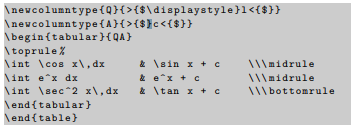
\includegraphics[scale=0.8]{1i.png}
			\end{figure}
		
		\subsection{article}
			
		
		\subsection{babel}
			O Latex pode ser configurado para escrever corretamente em muitos outros idiomas além do inglês, isso é um fator importante porque algumas línguas possuem características bem diferentes umas das outras, como o uso de hífenes, acentos, caracteres especiais, etc. O pacote babel do Latex fornece suporte à vários idiomas, incluindo o português do Brasil.
			Para usar o babel basta instalar o pacote do português como segue. \\
			sudo apt-get install texlive-lang-portuguese \\
			Depois é só inserir no inicio do documento a seguinte linha: \\
			$\backslash$usepackage[brazil]\{{babel}\}
		
		\subsection{beamer}
			Beamer é uma classe \LaTeX{} para produzir apresentações. Outras
			classes \LaTeX{} com o mesmo propósito são \emph{Seminar} e
			\emph{Prosper}. Ele possui recursos semelhantes aos encontrados no Prosper, permitindo
			desenvolver apresentações dinâmicas, com sobreposições (overlays)
			e transições animadas entre lâminas. As apresentações obtidas são arquivos \emph{pdf} que podem ser
			visualizadas no \emph{Acrobat Reader}.Isto torna as	apresentações altamente portáveis.
			Para usar a classe Beamer deve-se instalar o pacote apropriado
			disponível em $\backslash$url{http://latex-beamer.sourceforge.net/}. Também é
			necessário instalar os pacotes \emph{pgf} e \emph{xcolor}. Importante
			observar que Beamer e \LaTeX{} são necessários apenas para o
			desenvolvimento das lâminas (\emph{slides}), não sendo necessários para
			a visualização da apresentação, quando basta o Acrobat Reader ou o xpdf.
			Para usar a classe declara-se
			\verb+\documentclass{beamer}+ no início do arquivo \TeX. Beamer aceita
			a estruturação do texto usando \verb+\section+ e
			\verb+\subsection+. Slides individuais são definidos dentro de
			\verb+\frame{ ... }+ ou \verb+\begin{frame} ... \end{frame}+.
			
			Para produzir o arquivo final da apresentação, em formato pdf, não
			compilamos o arquivo
			usando \LaTeX{}, e sim usamos o programa \emph{pdflatex} (amplamente
			disponível nas instalações \TeX{} típicas) que converte diretamente o
			arquivo \TeX{} para \emph{pdf}.
		
		\subsection{biblatex}
			Para usar bibliografia no LaTeX precisamos utilizar o pacote biblatex e um arquivo com o nome refs.bib, por exemplo. Veja um exemplo do conteúdo deste arquivo:\\
			\begin{figure}[h]
				\centering
				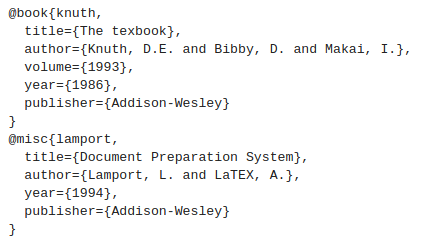
\includegraphics[scale=0.5]{2i.png}
			\end{figure}
			\newpage
			Para usar a BibTeX digite no final do documento, antes de $\backslash$end\{{document}\}.
			\begin{figure}[h]
				\centering
				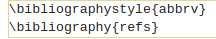
\includegraphics[scale=0.8]{3i.png}
			\end{figure}
		
		
		\subsection{bm}
			O pacote bm define um comando \ bm que torna seu argumento em negrito. O argumento pode ser qualquer objeto matemático de um único símbolo para uma expressão. Isto está intimamente relacionado com a especificação do comando \ boldsymbol no AMS-LATEX, mas o \ bm é mais cuidadoso na forma como faz as coisas.
			\begin{figure}[h]
				\centering
				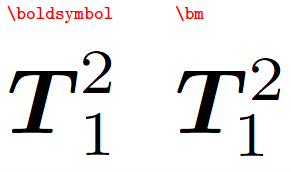
\includegraphics[scale=0.6]{6i.png}
			\end{figure}
		
		
		\subsection{booktabs}
			O pacote melhora a qualidade das tabelas no LATEX, fornecendo comandos extras e otimizações por trás dos bastidores. Diretrizes são dadas sobre o que constitui uma boa mesa neste contexto. A partir da versão 1.61, o pacote oferece compatibilidade com longtable. Segue exemplo abaixo:
			\begin{figure}[h]
				\centering
				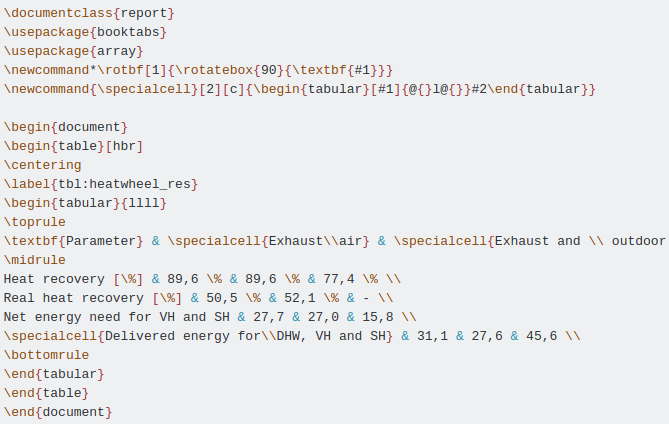
\includegraphics[scale=0.6]{5i.png}
			\end{figure}
			\newpage
		
		\subsection{color}
			A maneira mais simples de usar cores em seu documento LATEX é importando a cor do pacote ou xcolor. Ambos os pacotes fornecem um conjunto comum de comandos para manipulação de cores, mas o último é mais flexível e suporta um número maior de modelos de cores, portanto, é a abordagem recomendada. Abaixo um exemplo:
			\begin{figure}[h]
				\centering
				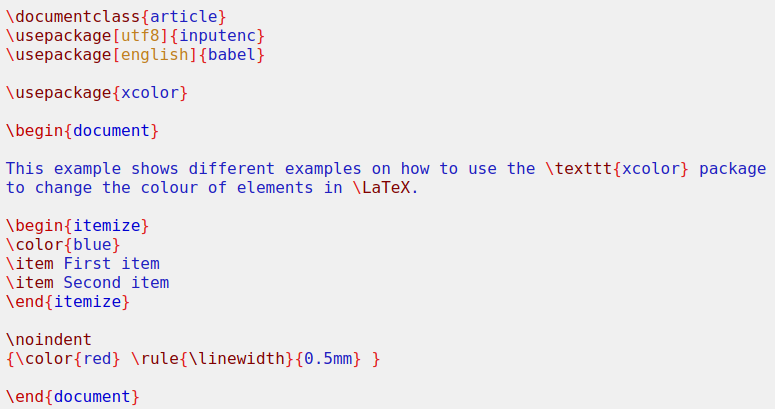
\includegraphics[scale=0.5]{4i.png}
			\end{figure}
			\newpage
			
			
		\subsection{dcolumn}
			O pacote dcolumn faz uso do pacote de matriz para definir um formato de coluna "D" para uso em ambientes tabulares. Basicamente, ele pode ser usado para  efetuar alinhamento dos pontos decimais na tabela do documento. Abaixo segue um exemplo da sua utilização para a criação de um tipo de tabela "D" (o último argumento é o numero de casas decimais):
			
			\begin{figure}[!htb]
				\centering
				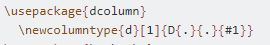
\includegraphics[scale=1]{dcolumn1.JPG}
			\end{figure}
			
			Este pacote faz parte do pacote latex-tools na distribuição necessária do \LaTeX.
		
		\subsection{enumitem}
			Um pacote para personalizar as três listas básicas (enumerar, itemize e description) por meio de um conjunto de parâmetros. Ele fornece funções para calcular o layout de rótulos e 'clonar' os ambientes padrão, para criar novos ambientes com seus próprios contadores. A seguir, são expostos alguns exemplos de usualidade do pacote:
			
			Para remover o espaço vertical completamente em uma lista:
			
			\begin{figure}[!htb]
				\centering
				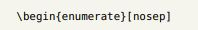
\includegraphics[scale=1]{2.JPG}
			\end{figure}
			
			Para iniciar o rótulo na margem e o texto do item no parindente atual:
			
			\begin{figure}[!htb]
				\centering
				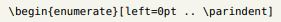
\includegraphics[scale=1]{3.JPG}
			\end{figure}
			
			Para definir um rótulo numérico com parênteses, mas uma referência cruzada sem eles:
			
			\begin{figure}[!htb]
				\centering
				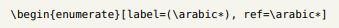
\includegraphics[scale=1]{4.JPG}
			\end{figure}
		
		
		\subsection{epsf}
			Este arquivo contém macros TEX para incluir um gráfico PostScript encapsulado. isto
			funciona encontrando o comentário da caixa delimitadora, calculando os valores de escala corretos e
			inserindo uma vbox do tamanho apropriado na posição atual no documento TEX.
			Para usar, digite em algum lugar no início do seu arquivo TEX:
			
			\begin{figure}[!htb]
				\centering
				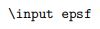
\includegraphics[scale=1]{5.JPG}
			\end{figure}
			
			Onde você desejar inserir um vbox para uma figura,use:
			
			\begin{figure}[!htb]
				\centering
				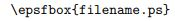
\includegraphics[scale=1]{6.JPG}
			\end{figure}
			
			Como alternativa, você pode fornecer sua própria caixa delimitadora:
			
			\begin{figure}[!htb]
				\centering
				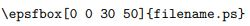
\includegraphics[scale=1]{7.JPG}
			\end{figure}
			
			Você pode ampliar ou reduzir a figura usando:
			
			\begin{figure}[!htb]
				\centering
				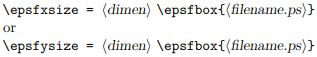
\includegraphics[scale=1]{8.JPG}
			\end{figure}
			
			Para usuários de \LaTeX, o pacote é hoje (bastante) obsoleto em favor do conjunto de pacotes latex-graphics \LaTeX mais sofisticados.
		
		\subsection{espfig}
			Usado para incluir Postscript Encapsulado em documentos L A T E X.
			Este pacote foi desenvolvido como uma solução geral para o problema de incluir gráficos em L A T E X 2.09. Essas versões antigas não devem ser usadas com L A T E X atuais.
			A solução atual 'preferida' é o pacote graphicx do L A T E X , mas o pacote gráfico contém uma versão do epsfig para uso com o L A T E X atual.
			
			Quando você usa LaTeX 2.09, insira a seguinte linha no começo: documentstyle... 
			\begin{figure}[!htb]
				\centering
				
\includegraphics[scale=1.1]{9.JPG}
			\end{figure}
			
			No ponto em que você deseja incluir a figura, escreva:
			\begin{figure}[!htb]
				\centering
				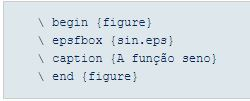
\includegraphics[scale=1.1]{10.JPG}
			\end{figure}
			
			Naturalmente, você deve substituir o nome do arquivo e a legenda da figura pelos que você precisa. Você também pode alterar o tamanho da figura usando os comandos:
			\begin{figure}[!htb]
				\centering
				
\includegraphics[scale=1.1]{11.JPG}
			\end{figure}
			
			Em LaTeX2e (onde lê a primeira linha do documento ), adicione a seguinte linha: documentclass...
			
			\begin{figure}[!htb]
				\centering
				
\includegraphics[scale=1.1]{12.JPG}
			\end{figure}
			
			No ponto em que você deseja incluir a figura, coloque:
			\begin{figure}[!htb]
				\centering
				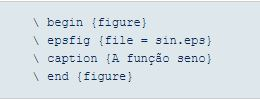
\includegraphics[scale=1.1]{13.JPG}
			\end{figure}
			
			Para dimensionar o gráfico e / ou para girá-lo, adicione os argumentos width, height ou angle como mostrado abaixo:
			\begin{figure}[!htb]
				\centering
				
\includegraphics[scale=1.1]{14.JPG}
			\end{figure}
		
		\subsection{fancyhdr}
			Controle extensivo de cabeçalhos e rodapés de página em L A T E X2e.
			O pacote oferece instalações extensas, tanto para construir cabeçalhos e rodapés, quanto para controlar seu uso (por exemplo, às vezes, quando L A T E X mudaria automaticamente o estilo de cabeçalho em uso).
			
			O que o Fancyhdr permite é definir um estilo que usamos depois com o (contra barra)thispagestyle
			Um exemplo de seu uso será mostrado a seguir.
			
			Então imaginemos que todas as páginas vão ter no cabeçalho: o título à esquerda e o autor à direita e no rodapé: a página à direita, definimos no preâmbulo todas essas instruções:
			\begin{figure}[!htb]
				\centering
				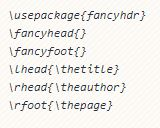
\includegraphics[scale=1.1]{15.JPG}
			\end{figure}
		
		\subsection{geometry}
			Interface flexível e completa para documentar dimensões.
			O pacote fornece uma interface de usuário fácil e flexível para personalizar o layout da página, implementando mecanismos de autocentralização e balanceamento automático para que os usuários tenham apenas que fornecer a menor descrição possível para o layout da página. Por exemplo, se você deseja definir cada margem de 2 cm sem espaço de cabeçalho, o que você precisa é apenas (contra barra)\ usepackage [margin = 2cm, nohead] {geometry} .
			
			O pacote conhece todos os tamanhos de papel padrão, de modo que o usuário não precisa saber quais são as dimensões nominais "reais" do papel, apenas seu nome padrão (como a4 , carta,etc.).
			Uma característica importante é a capacidade do pacote de comunicar o tamanho do papel que está configurado para a saída (seja via DVI (contra barra)\ special s ou via interação direta com o pdf (La ) T e X ).
			
			Este pacote fornece uma interface flexível e fácil para as dimensões da página. Você pode mudar a página layout com parâmetros intuitivos. Por exemplo, se você quiser definir uma margem a 2cm de cada borda o papel, você pode digitar apenas:
			\begin{figure}[!htb]
				\centering
				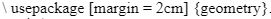
\includegraphics[scale=1.1]{17.JPG}
			\end{figure}
			
			
			Alterar o layout de página no meio do documento. Os novos comandos(contra barra) \ newgeometry {· · ·} e (contra barra)\ restoregeometry permitem que os usuários alterem a dimensão da página. no meio do documento. (contra barra)\ newgeometry é quase similar a (contra barra)\ geometry exceto que (contra barra)\ newgeometry desabilita todas as opções especificadas no preâmbulo e ignora as propriedades relacionadas ao opções: paisagem, retrato e opções de tamanho de papel (como papersize, paper = a4paper e assim adiante).
			
			Para definir as dimensões do layout da página em L A TEX não é simples. Você precisa ajustar vários L A TEX dimensões nativas para colocar uma área de texto onde você deseja. Se você quiser centralizar a área de texto no papel você usa, por exemplo, você tem que especificar dimensões nativas como segue:
			\begin{figure}[!htb]
				\centering
				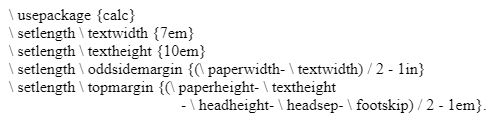
\includegraphics[scale=1.1]{16.JPG}
			\end{figure}
		
		\subsection{graphics}
			O pacote foi projetado para acomodar todas as necessidades de inclusão de gráficos em documentos L A T E X , substituindo muitos pacotes anteriores usados em L A T E X 2.09. O pacote tem como objetivo fornecer uma interface consistente para incluir os tipos de arquivos compreendidos em sua saída, usando 'drivers de impressora' (agora conhecidos simplesmente como 'drivers'). 
			
			A distribuição do pacote contém vários drivers, mas outros (por exemplo, pdf T E X) são distribuídos separadamente. O pacote também oferece vários meios de manipular gráficos no decorrer da inserção deles em um documento (por exemplo, rotação e dimensionamento).
			Para documentação estendida, veja epslatex .
			
			O pacote faz parte do pacote gráfico , que é uma das coleções no pacote de pacotes 'requerido' L A T E X.
			
			Para incluir um arquivo gráfico:
			\begin{figure}[!htb]
				\centering
				\includegraphics[scale=1.1]{18.JPG}
			\end{figure}
		
		\subsection{graphicx}
			Suporte aprimorado para gráficos.
			O pacote se baseia no pacote graphics , fornecendo uma interface de valor-chave para argumentos opcionais para o comando \ includegraphics . Essa interface fornece recursos que vão muito além do que o pacote graphics oferece por si só.
			Para documentação estendida, veja epslatex .
			O pacote faz parte do pacote latex-graphics , que é uma das coleções do pacote 'obrigatório' de L A T E X.
			
			Compatibilidade entre graphics e graphicx Para um autor de documentos, não há realmente nenhum problema de compatibilidade entre os dois pacotes. Você acabou de escolher a interface que você prefere, e, em seguida, use o pacote apropriado. Para um pacote ou redator de turma, a situação é um pouco diferente. Suponha que você está escrevendo uma classe de carta que precisa imprimir um logotipo da empresa como parte do papel timbrado. Como o autor da aula, você pode querer dar aos usuários a possibilidade de usar interface em suas letras (caso precisem incluir gráficos adicionais no corpo da carta). Neste caso, a classe deve carregar o pacote graphics (não graphicx, pois isso comprometeria quaisquer usuários da classe na interface keyval).
			
			
			Usando o graphicx, o primeiro passo a tomar é garantir que você tenha o comando:
			
			\begin{figure}[!htb]
				\centering
				\includegraphics[scale=1.1]{19.JPG}
			\end{figure}
			
			A importação de um gráfico é feita usando o comando:
			
			
			\begin{figure}[!htb]
				\centering
				\includegraphics[scale=1.1]{20.JPG}
			\end{figure}
		
		
		\subsection{hyperref}
			O pacote hyperref fornece ao LaTeX a capacidade de criar hyperlinks dentro do documento. Ele funciona com \textit{pdflatex} e também com o padrão "latex" usado com \textit{dvips} e \textit{ghostscript} ou \textit{dvipdfm} para construir um arquivo PDF. Se você carregá-lo, você terá a possibilidade de incluir links externos interativos e todas as suas referências internas serão transformadas em hiperlinks. O compilador \textit{pdflatex} torna possível criar arquivos PDF diretamente da fonte LaTeX, e o PDF suporta mais recursos que o DVI. Em particular, o PDF suporta hiperlinks. Além disso, o PDF pode conter outras informações sobre um documento, como o título, o autor, etc., que podem ser editadas usando o mesmo pacote.\\
			O uso básico com as configurações padrão é simples. Basta carregar o pacote no preâmbulo:
			\begin{figure}[h]
				\centering
				\includegraphics[scale=0.6]{caa.png}
			\end{figure}
		
			Isso automaticamente transformará todas as suas referências internas em hiperlinks. Isso não afetará a maneira de escrever seus documentos: basta continuar usando o padrão $\backslash$label- $\backslash$refsistema (discutido no capítulo sobre etiquetas e referências cruzadas); com hyperref essas "conexões" se tornarão links e você poderá clicar neles para ser redirecionado para a página correta. 
			\newpage
			Além disso, o índice, a lista de figuras $\backslash$ tabelas e o índice serão também feitos de hiperlinks. Os hiperlinks não serão exibidos se você estiver trabalhando no modo de rascunho.\\
			Exemplo 1:
			\begin{figure}[h]
				\centering
				\includegraphics[scale=0.5]{ref.png}
			\end{figure}
		
			Exemplo 2: 
			\begin{figure}[h]
				\centering
				\includegraphics[scale=0.6]{si.png}
			\end{figure}
		
			Exemplo 3:
			\begin{figure}[h]
				\centering
				\includegraphics[scale=0.6]{f.png}
			\end{figure}
		
		\subsection{latexsym}
			O pacote latexsym fornece 11 símbolos matemáticos que foram originalmente definidos no LaTeX2.09, mas não são mais definidos no Esquema de Seleção de Novas Fontes. 
			Esses símbolos também são fornecidos pelos pacotes amsfonts e amssymb. Como o SWP e o SW chamam o pacote amsfonts automaticamente, normalmente você não precisa adicionar o pacote latexsym ao seu documento para obter os símbolos. Nenhuma opção de pacote está disponível. O pacote latexsym está instalado no diretório base TCITeX / TeX / LaTeX /. O site para download é:\\
			https://www.mackichan.com/index.html?techtalk/500.htm~mainFram\\ e o arquivo deve estar armazenado na mesma pasta dos arquivos LaTeX.
		
		\subsection{listings}
			Usando as listagens de pacotes, você pode adicionar texto não formatado como faria com, mas seu objetivo principal é incluir o código-fonte de qualquer linguagem de programação em seu documento. Para usar o pacote, você precisa:\\
			\begin{center}
				$\backslash$usepackage \{{ listagens }\}
			\end{center}
			O pacote de listagens suporta o destaque de todos os idiomas mais comuns e é altamente personalizável. Se você quiser apenas escrever código em seu documento, o pacote fornece o ambiente lstlisting:\\
			Exemplo 1:
			\begin{figure}[h]
				\centering
				\includegraphics[scale=0.6]{dd.png}
			\end{figure}\\
			Exemplo 2:
			\begin{figure}[h]
				\centering
				\includegraphics[scale=0.6]{py.png}
			\end{figure}\\
			Exemplo 3:
			\begin{figure}[h]
				\centering
				\includegraphics[scale=0.4]{do.png}
			\end{figure}
		
		\subsection{microtype}
			Este pacote faz pequenos ajustes na distribuição, tamanho e forma das letras em cada linha de maneira que o texto esteja alinhado à esquerda e à direita simultaneamente sem introduzir espaçamento excessivo entre as palavras e com uma apresentação agradável, facilitando a leitura. Para usar o pacote, você precisa:\\
			\begin{center}
				$\backslash$usepackage\{{microtype}\}
			\end{center}
			Exemplo 1:\\
			\begin{center}
				$\backslash$usepackage[tracking=alltext,letterspace=-40]{microtype}
			\end{center}
			Exemplo 2:\\
			\begin{center}
				$\backslash$usepackage[protrusion=allmath,tracking=smallcaps]\{{microtype}\}
			\end{center}
		
		\subsection{multicol}
			Se você está escrevendo um texto em uma única coluna e quer que parte dele apareça em mais colunas, você
			pode fazer isso usando o pacote \textit{multicol}. Para isso basta colocar no preâmbulo o comando:\\
			\begin{center}
				$\backslash$usepackage\{{multicol}\}
			\end{center}
			Com esse pacote podemos escrever textos não só em 2 colunas, como também em 3, 4, . . . Par isso escreva
			o texto que irá aparecer em várias colunas de $\backslash$begin \{{multicols}\}\{{n}\} e $\backslash$end\{{multicols}\}, e no lugar de n coloque o número de colunas que você quer. Por exemplo, digitando o texto:
			\begin{figure}[h]
				\centering
				\includegraphics[scale=0.8]{co.png}
			\end{figure}
		
			e o texto vai aparecer assim:
		
			\begin{figure}[h]
				\centering
				\includegraphics[scale=0.7]{exp.png}
			\end{figure}
			Tudo que for digitado depois de $\backslash$end\{{multicols}\} volta a ser apresentado em uma única coluna.
		
		\subsection{revtex/revtex4}
			REVTeX é um conjunto de pacotes para serem usados com LaTeX2e. A primeira versão foi lançada em 1986. A quarta versão, REVTeX 4, em 2001. A
			versão atual é a REVTeX 4.1. Estes pacotes são destinados à redação de artigos para a submissão
			nas revistas da APS e AIP.\\
			Para realizar a instalação basta seguir o passo a passo:\\
			\begin{itemize}
			
				\item Baixe revtex4-1.zip do seguinte endereço: https://authors.aps.org/revtex4/
				\item Extraia revtex4-1.zip e dentro desta pasta abra o terminal
				\item No terminal copie e cole:  “sudo unzip revtex4-1-tds.zip -d /etc/texmf”
				\item Para incluir o pacote  revtex4-1 em seu documento latex adicione: $\backslash$documentclass [preprintnumbers,amsmath,amssymb,pre,floatfix]\{{revtex4-1}\}
			
			\end{itemize}
			Exemplo:
			
			\begin{figure}[h]
				\centering
				\includegraphics[scale=0.6]{re.png}
			\end{figure}
		
		
		\subsection{times}
			O pacote times já é obsoleto devido ao bug do escalamento das fontes. Em vez do times, use a combinação de mathptmx, helvet, e courier ($\backslash$usepackage\{{math\\ptmx,courier}\} $\backslash$usepackage[scaled=.92]{helvet}) em vez do times para mapear fontes para ser compatíveis com o times: Adobe Times para roman (fonte de espaçamento variável para corpo do texto) e  math (fórmula), Helvetica para Sans Serif (fontes sem a serifa), Courier para typewriter (fontes mono espaçados para códigos). Note que a fonte typewriter é mais fino que demais fontes e as fontes e símbolos adicionais tais como fontes do AMS, Black board bold fonts, etc, não serão oferecidos e eles podem ficar como no original (normalmente, compatível com a fonte Computer Modern).  Para ter fontes tudo compatíveis com times, opte pelo pacote txfonts.\\
			Para usar o pacote, você precisa:\\
		
			\begin{center}
				$\backslash$usepackage\{{times}\}
			\end{center}
		
		
	
\end{document}